\documentclass[10pt,journal,compsoc]{IEEEtran}
% *** CITATION PACKAGES ***
%
\let\labelindent\relax
\usepackage{enumitem}
\usepackage{url}
\ifCLASSOPTIONcompsoc
  % IEEE Computer Society needs nocompress option
  % requires cite.sty v4.0 or later (November 2003)
  % \usepackage[nocompress]{cite}
\else
  % normal IEEE
  % \usepackage{cite}
\fi

\makeatletter
% Label with name
\def\namedlabel#1#2{
  \label{#1}
  \begingroup
   \def\@currentlabel{#2}%
   \label{#1:name}\endgroup
}

% Label with name and displayed
\def\nameddisplayedlabel#1#2{
  \label{#1}
  \begingroup
   \def\@currentlabel{#2}%
   \label{#1:name}\endgroup
   \textbf{#2}\hfill\\
}

% Reference with name
\def\namedref#1{\ref{#1} \ref{#1:name}}
\makeatother



% *** GRAPHICS RELATED PACKAGES ***
%
\ifCLASSINFOpdf
   \usepackage[pdftex]{graphicx}
  % declare the path(s) where your graphic files are
  % \graphicspath{{../pdf/}{../jpeg/}}
  % and their extensions so you won't have to specify these with
  % every instance of \includegraphics
  % \DeclareGraphicsExtensions{.pdf,.jpeg,.png}
\else
  % or other class option (dvipsone, dvipdf, if not using dvips). graphicx
  % will default to the driver specified in the system graphics.cfg if no
  % driver is specified.
   \usepackage[dvips]{graphicx}
  % declare the path(s) where your graphic files are
  % \graphicspath{{../eps/}}
  % and their extensions so you won't have to specify these with
  % every instance of \includegraphics
  % \DeclareGraphicsExtensions{.eps}
\fi



\hyphenation{op-tical net-works semi-conduc-tor crea-ted NajNaf}


\begin{document}
%
% paper title
% can use linebreaks \\ within to get better formatting as desired
\title{NajNaf: WantCloud BV's Large Scale Image Resizer}
\author{\IEEEauthorblockN{F.W. Bakker\IEEEauthorrefmark{1}}
\and
\IEEEauthorblockN{S.F. van Wouw\IEEEauthorrefmark{1}}

\and
\IEEEauthorblockN{prof.dr.ir. D.H.J. Epema\IEEEauthorrefmark{2}}
\and
\IEEEauthorblockN{dr.ir. A. Iosup\IEEEauthorrefmark{2}}
\and
\IEEEauthorblockN{ir. B.I. Ghit\IEEEauthorrefmark{3}}\\\hfill\\
\and

\IEEEauthorblockA{\IEEEauthorrefmark{1}Authors
\{f.w.bakker,s.f.vanwouw\}@student.tudelft.nl\\
\IEEEauthorrefmark{2}Instructors \{d.h.j.epema,a.iosup\}@tudelft.nl\\
\IEEEauthorrefmark{3}Lab Assistant b.i.ghit@tudelft.nl}

}
%\author{Fritsjan Bakker 1527045 and Stefan van Wouw 1543776}% <-this % stops a space
% for Computer Society papers, we must declare the abstract and index terms
% PRIOR to the title within the \IEEEcompsoctitleabstractindextext IEEEtran
% command as these need to go into the title area created by \maketitle.
\IEEEcompsoctitleabstractindextext{%
\begin{abstract}
%\boldmath
WantCloud BV's current image resizing and persistant storage system is not able
to cope with peak loads and does not scale up or down without human
intervention.
In this paper NajNaf is proposed: a system that is scalable, reliable, and durable
without human intervention. The system is implemented as a cloud based
application and has different subsystems that can be hosted in different virtual
machines. This service oriented approach makes it possible to independently
scale different parts of the system when necessary.
Experiments with a prototype of the system on the DAS-4 cluster of the Delft
University of Technology show that NajNaf dynamically scales
up and down. This results in more than 90\% of the tasks finishing before the global
deadline. NajNaf ensures reliability by introducing redundance into the
system. It therefore is a viable alternative to the current system.

\end{abstract}
% IEEEtran.cls defaults to using nonbold math in the Abstract.
% This preserves the distinction between vectors and scalars. However,
% if the journal you are submitting to favors bold math in the abstract,
% then you can use LaTeX's standard command \boldmath at the very start
% of the abstract to achieve this. Many IEEE journals frown on math
% in the abstract anyway. In particular, the Computer Society does
% not want either math or citations to appear in the abstract.

% Note that keywords are not normally used for peerreview papers.
}


% make the title area
\maketitle


\section{Introduction}
% Introduction (recommended size, including points title page and abstract: 1
% page): describe the problem, the existing systems and/or tools (related work),
% the system you are about to implement, and the structure of the remainder of
% the article; use one short paragraph for each.
% Why what how and
WantCloud BV has an application that resizes and stores images in one relational database
hosted by a shared webhosting provider. This system has one main issue: it does
not scale automatically with the amount of concurrent users. Therefore the
system cannot deal with peak loads efficiently. In addition, the relational
database quickly becomes the bottleneck, because it has only one entry point.

In order to deal with the problems the current system has, a new system is
proposed: NajNaf, of which the design is described in this paper.
NajNaf is a large scale image resizer with persistent storage support that is
specifically designed to be scalable, reliable, and durable without requiring
human intervention. As such, this system deals with the problems WantCloud
BV's current system has. 

NajNaf can be hosted on a cloud infrastructure like Amazon
EC2\footnote{ Amazon EC2 \url{http://aws.amazon.com/ec2/}} or on a grid
computing infrastructure like 
DAS-4\footnote{DAS-4 (The Distributed ASCI Supercomputer 4)
\url{http://www.cs.vu.nl/das4/home.shtml}}. The system has different subsystems
which each can be hosted on a separate VM (Virtual Machine). The head node
subsystem is responsible for monitoring all other
subsystems, and scaling their capacity up or down when necessary. The master
node is responsible for taking all image resize tasks and keeps track of them in a
queue. The worker node subsystem consumes multiple image resize tasks off the master's
queue and executes them parallel. Finally the persistent storage subsystem stores the resized images
in a distributed object database.

If a subsystem fails it is automatically replaced by a new VM running this
subsystem. In case of the master this is a mirrored version (so the tasks in the
queue do not get lost), and in case of a worker it is a new worker, after which
the master automatically reschedules the lost image tasks.

Experiments with a prototype of the system (not implementing persistent storage) were conducted on the DAS-4 cluster using VMs with one cpu core
available each. The experiments show that the system reacts to load changes and
creates or suspends VMs accordingly within 15 seconds after the load change.
This results in more than 90\% of the tasks finishing before the global
deadline.


The remainder of the paper is structured as follows:
In section \ref{sec:requirements} 
requirements of the system are described, followed by the system design
in section \ref{sec:System Design}. The performance of the system is
evaluated in section \ref{sec:Experimental
Results}. Lastly, the pros and cons of the cloud based approach are evaluated in section
\ref{sec:Discussion} and conclusions are in \ref{sec:Conclusion}.



% (recommended size: title + abstract + intro = 1 page)
% describe the problem, the existing systems and/or tools (related work), the
% system you are about to implement, and the structure of the remainder of the
% article; use one short paragraph for each.

\section{Requirements}
\label{sec:requirements}
% recommended size: 0.5 pages): describe the application (1
% paragraph) and its requirements (1-3 paragraphs, summarized in a table if
% needed).
There are two sets of requirements to the system: the requirements for the production system and
the requirements for the prototype system. In this section we will first list
the requirements of the prototype followed by the list of requirements
for the production system. Note that the second list is an extension of the first
list - all prototype requirements are also requirements for the production system.
Functional requirements are annotated with \emph{FR}, while non-functional
requirements (constraints) are annotated with \emph{NFR}.\\

\noindent\textbf{Prototype system:}
\begin{enumerate}[leftmargin=1.5cm,label={[FR:\arabic*]}]
  \item\nameddisplayedlabel{fr:resize-image}{Image Resizing}
  The system should resize the images such that they fit into the following
  dimension boxes (keeping aspect
  ratio intact): $128 \times 128$, $512 \times 512$ and $1024 \times 1024$
  (customizable by customer).
  \item\nameddisplayedlabel{fr:monitoring}{Monitoring}
The system should include a monitoring-subsystem allowing
        administrators an insight into the performance of the system.
    \end{enumerate}
\begin{enumerate}[leftmargin=1.5cm,label={[NFR:\arabic*]}]
  \item\nameddisplayedlabel{nfr:automation}{Automation}
    Running the system should not require any human intervention.
  \item\nameddisplayedlabel{nfr:elasticity}{Elasticity}
Upon a higher load the system's capacity must be automatically increased. When
the load lowers the capacity must be reduced to minimize costs.
  \item\nameddisplayedlabel{nfr:load-balancing}{Load Balancing (Performance)}
  The system should evenly distribute the tasks over the available VMs.
  \item\nameddisplayedlabel{nfr:modularity}{Modularity}
  The system should have a Service Oriented Architecture (SOA) in order to be
  able to re-use different components within other WantCloud BV systems. 
  \item\nameddisplayedlabel{nfr:reliability}{Reliability}
Downscaling the system (removing VMs) should not cause tasks to be
        dropped. Nor should tasks be dropped when a part of the system fails.
        Single point of failures are still allowed in the system (master and
        head node, see section
        \ref{sec:System Design}).
  \item\nameddisplayedlabel{nfr:response-time}{Response time}
      The time from when an image task is submitted until it has been completed
      should not exceed the global deadline of 30 seconds for at least 90\% of
      all tasks.
    \end{enumerate}

\noindent\textbf{Production system:}
\begin{enumerate}[leftmargin=1.5cm,label={[FR:\arabic*]},start=3]
  \item\nameddisplayedlabel{fr:persistent-storage}{Persistent Storage}
  The resized images should be saved into a persistent storage facility.
  \end{enumerate}
\begin{enumerate}[leftmargin=1.5cm,label={[NFR:\arabic*]},start=7]
  \item\nameddisplayedlabel{nfr:durability}{Durability}
  The persistent storage should make sure the stored images do not perish.
  \item\nameddisplayedlabel{nfr:no-spof}{No single point of failure}
    The system must be even more reliable by removing all single point of
        failures - all subsystems must support some form of replication.
  \item\nameddisplayedlabel{nfr:fairness}{Multi-tenancy Fairness}
    The system must ensure the system is fair which is defined as: Users
    submitting first get served first and no starvation should occur (e.g. when
    one user submits a lot of jobs at once the users after this user should
    still get their jobs completed within finite time).
    \end{enumerate}


\section{System Design}
\label{sec:System Design}
\subsection{Resource Management Architecture}
\label{ssec:Resource Management Architecture}
% describe the design of your system,
% including the inter-operation of the provisioning, allocation, reliability, and
% monitoring components (which correspond to the homonym features required
% by the WantCloud CTO).
\begin{figure*}
\centering
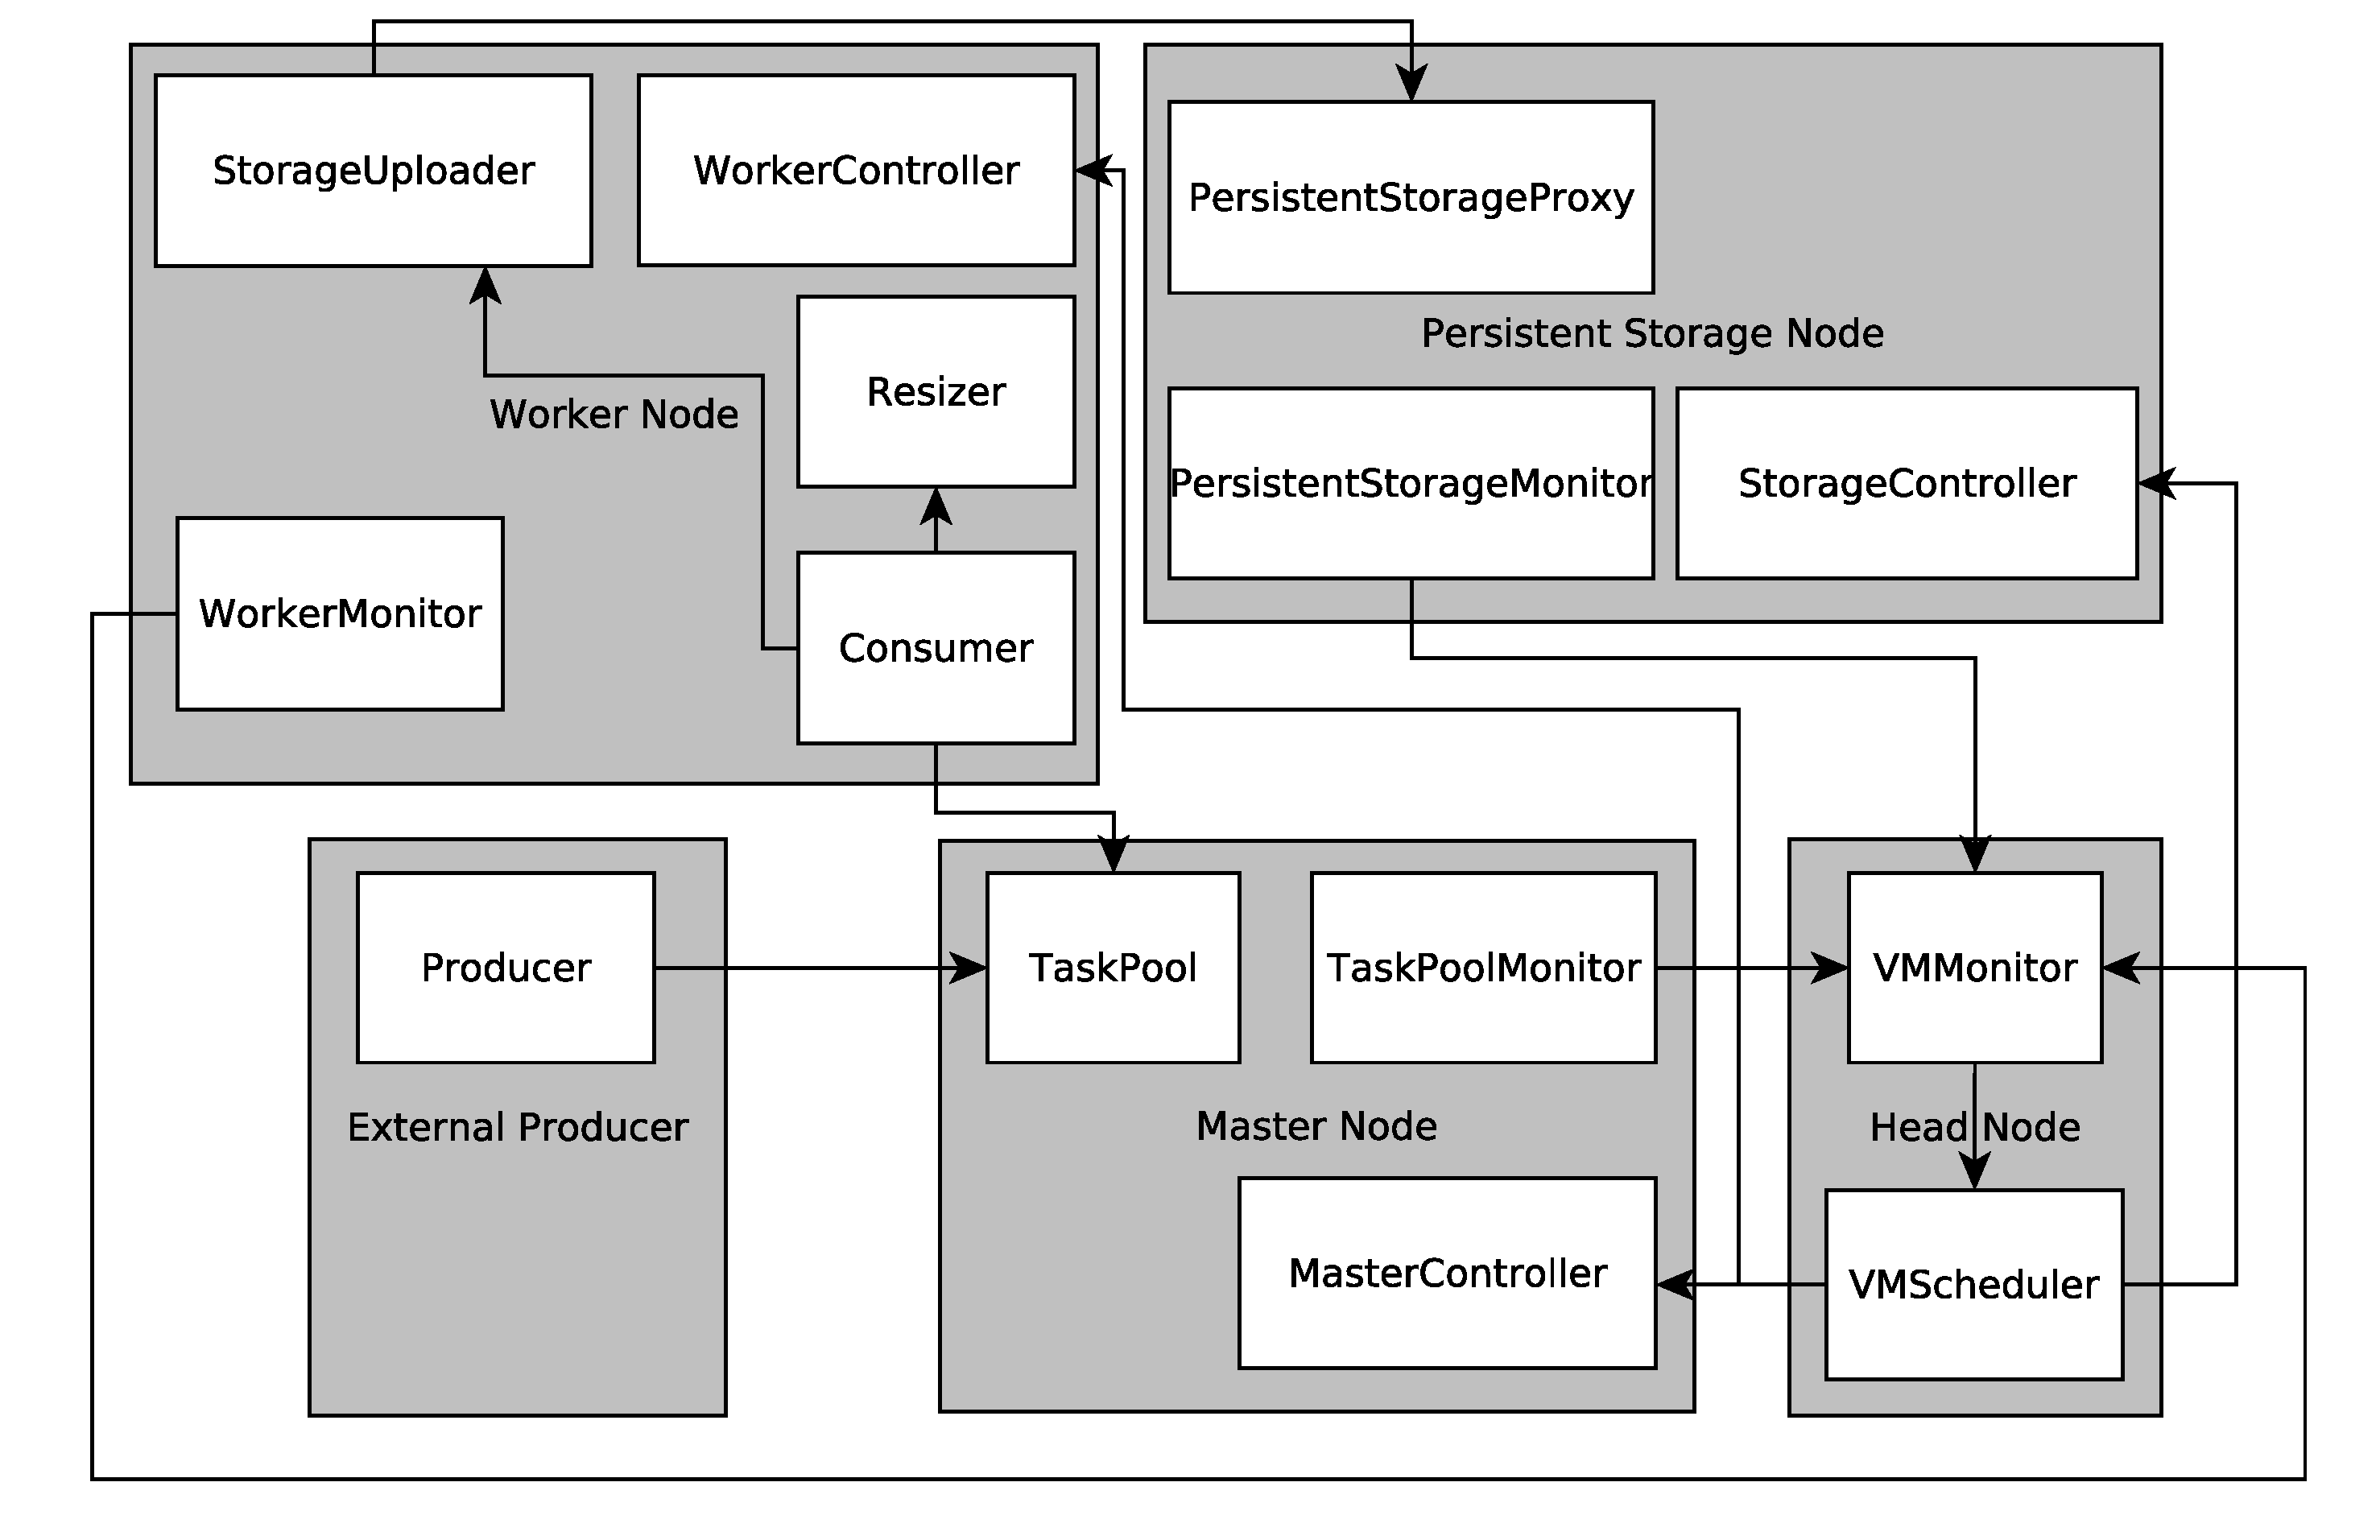
\includegraphics[width=0.9\linewidth]{system_design.pdf}
\caption{System Design to VM Type Mapping}
\label{fig:system-design}
\end{figure*}

%The \emph{Consumer} in each \emph{Worker Node} checks the system usage of the
%various workers it maintains. When the load is low enough it fetches another
%\emph{Task} from the \emph{TaskPool}. It then creates a thread and gives the
%\emph{Task} to this thread. It sends the usage of the system in a heartbeat to
%the \emph{VMWorker} on the \emph{Head Node}.

The global system design together with the allocation of system components to
different types of VMs is depicted in figure \ref{fig:system-design}.
Components are grouped together on one VM type based on their coherence (as one
would do when designing subsystems). However, components on the same VM type are
decoupled as much as possible (using interfaces), such that they can be
maintained independently (\namedref{nfr:modularity}).
The system is described per VM type below. By referring to the requirements
when explaining each component, one can infer whether the respective feature is
actually implemented or not\footnote{We have taken additional features such as
durability and multi-tenancy fairness into account but did not actually implement them in the prototype
version. We therefore did not include an \emph{additional features} section. We
consider the 
additional feature scheduling to been implemented by mechanic of section \ref{sssec:slow-start} and
the master-worker setup}.

\subsubsection{The Head Node}
\label{sssec:head-node}
The head node is responsible for managing all VMs (and itself is not a VM in our
setup). It has a \emph{VMMonitor} (\namedref{fr:monitoring})
which receives status updates from running VMs. The
\emph{VMScheduler} starts or stops VMs based on the feedback it receives from
the \emph{VMMonitor} (\namedref{nfr:elasticity}). This component is also responsible for the initial startup
of the entire system (\namedref{nfr:automation}).

\subsubsection{The Master Node}
The system uses a master-worker setup to process images. There is one
(possibly replicated, \ref{nfr:no-spof}) master, and there are multiple workers.
A master node hosts the \emph{TaskPool}, to which external producer programs
(depicted by the External Producer VM type in figure \ref{fig:system-design}) can
push their image resize tasks. This \emph{TaskPool} is implemented as a message
queue with FIFO ordering (or can be modified to use a certain priority rule,
depending on the fairness policy). The \emph{TaskPoolMonitor} sends
heartbeats to the \emph{VMMonitor} containing the current
resource utilization information and queue length. Finally the
\emph{MasterController} accepts commands from the \emph{VMScheduler} (such as:
prepare to shutdown).

\subsubsection{The Worker Nodes}
Multiple worker nodes are responsible for resizing images
and uploading them to the persistent storage (\namedref{fr:resize-image}). This is accomplished by a
single \emph{Consumer} per worker node that spawns a resize task thread for
every task consumed from the \emph{TaskPool}. When resizing has finished,
the \emph{StorageUploader} takes over and inserts the resized images into the
persistent storage (\namedref{fr:persistent-storage}). 

The \emph{WorkerController} is similar to the \emph{MasterController}. The
\emph{WorkerMonitor} reports the average image resize speed and the amount of
concurrent image resize tasks it is running to the \emph{VMMonitor}. 
The task of resizing and uploading to storage is considered
to be one atomic operation. The \emph{Consumer} will only acknowledge back to
the \emph{TaskPool} if the entire task succeeded.



\subsubsection{The Persistent Storage Nodes}
Multiple persistent storage node VMs are responsible for storing the (resized)
images (\namedref{fr:persistent-storage}). The \emph{PersistentStorageProxy} is aware of the exact partitioning of
persistent storage shards of a distributed object database such as
CouchDB\footnote{An example of how this can be accomplished with CouchDB can be
found at \url{http://guide.couchdb.org/editions/1/en/clustering.html}}. Replicating
database clusters ensures \namedref{nfr:durability}.


The
\emph{PersistentStorageMonitor} and \emph{StorageController} are based on the
same idea as the \emph{TaskPoolMonitor} and \emph{MasterController}. The first
sends heartbeats to the \emph{VMMonitor}, and the latter accepts commands from
the \emph{VMScheduler}.


\subsubsection{States and Commands}
The worker and master's application state is used to inform the head node of 
the state the application is in (this state is important when the respective VM
is actually up and running). Figure \ref{fig:app_state} shows the state diagram of
the worker. The labels along the edges of the state diagram show what is
required for the application to switch states. The `err' is an 
internal event, while \texttt{INIT} and \texttt{SHUTDOWN} are commands received from the head
node. A typical usage pattern is to send an \texttt{INIT} command with the
master's ip address to a worker in the \texttt{READY} state. And a
\texttt{SHUTDOWN} command when the worker is no longer needed, after which the
worker can be suspended if the worker enters the \texttt{READY} state again. If
the head node detects a worker in the \texttt{ERROR} state, it will try to
reset the worker by resending an \texttt{INIT} command. If this fails it simply
deletes the worker.

\begin{figure*}
\centering
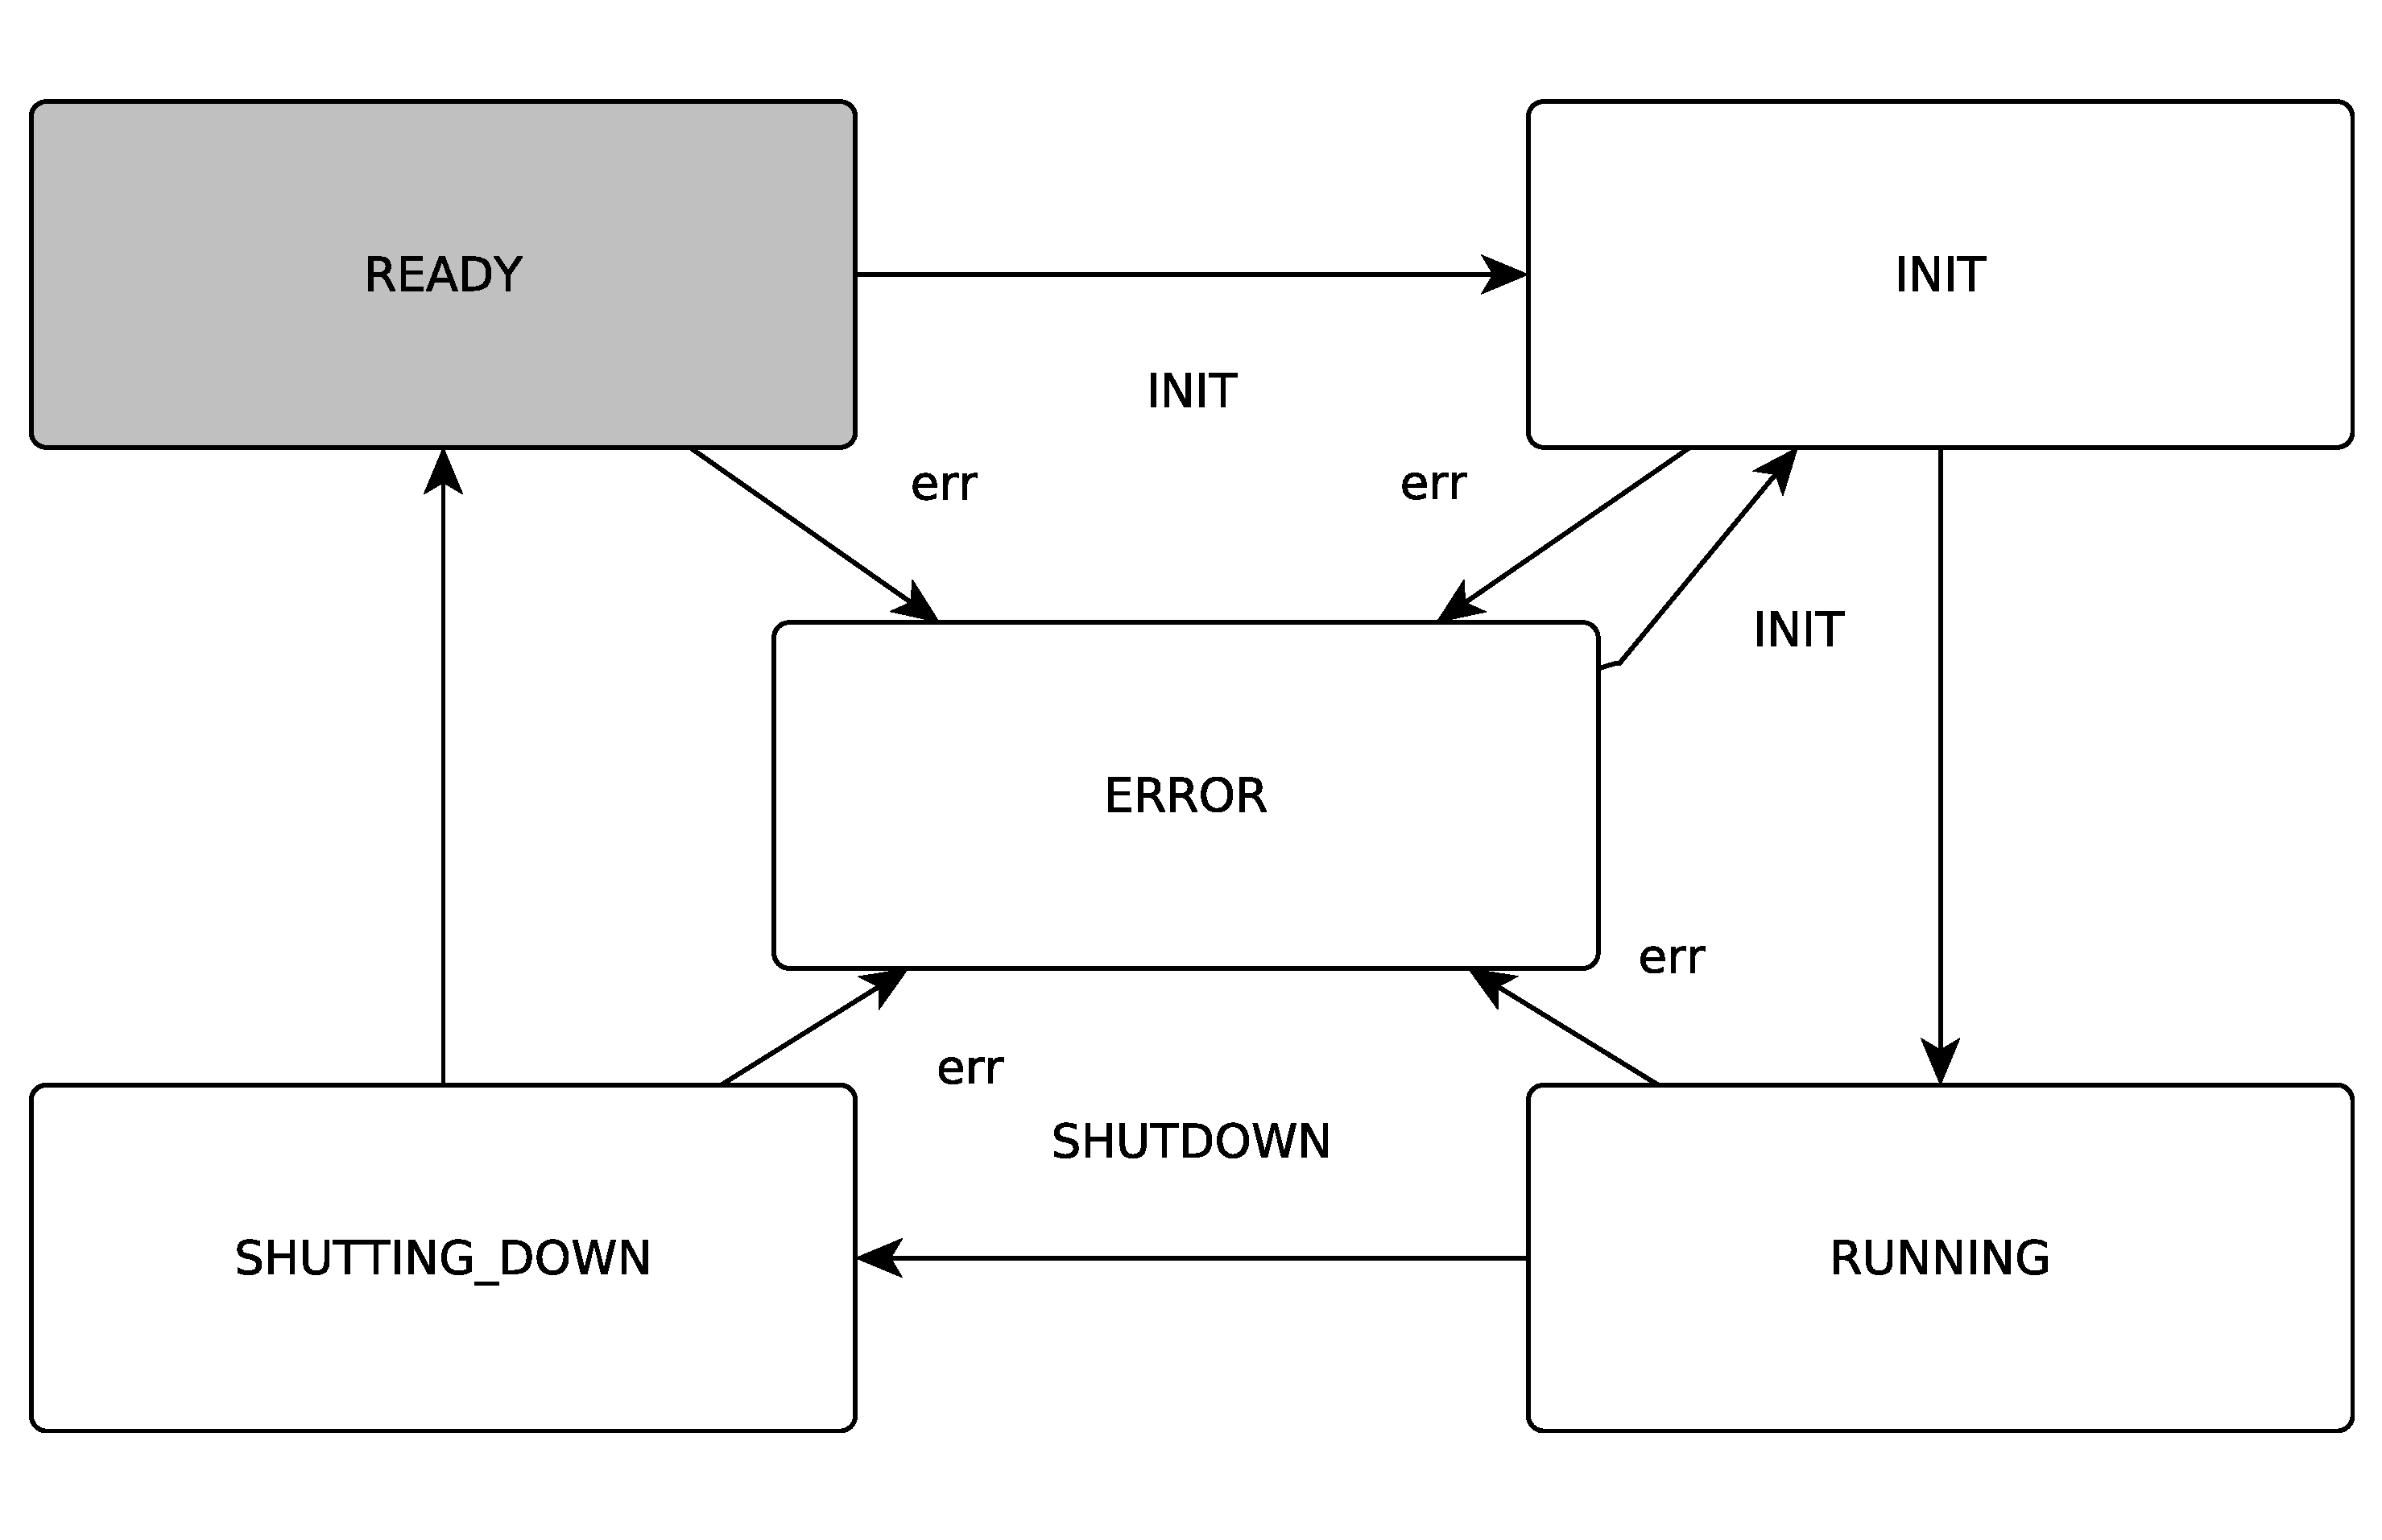
\includegraphics[width=0.9\textwidth]{app_state_v2.pdf}
\caption{State diagram of the worker}
\label{fig:app_state}
\end{figure*}


\subsection{System Policies}
\label{ssec:System Policies}
The system has different policies in place in order to comply with constraints set in
section \ref{sec:requirements}. These are explained in the sections below.

\subsubsection{Scaling}
The system is able to automatically scale up and down when needed
(\namedref{nfr:elasticity} and \namedref{nfr:automation}). In the current design
the persistent storage only scales up, and the worker nodes can scale up and
down. The master node does not scale (it is assumed it can handle the queue on
its own).

All VMs
periodically send
heartbeats with their current resource utilization to the 
\emph{VMMonitor}. The monitor keeps track of the most recent heartbeats and
periodically sends them to the \emph{VMScheduler} (this means heartbeats can
arrive in a certain timespan, resulting in a synchronised mechanism). The
\emph{VMScheduler} in turn will use the heartbeat data to determine what
commands to issue (if any).

The \emph{VMScheduler} will decide to scale up (add more worker nodes) if
the total expected time it takes to process all image tasks in the
\emph{TaskPool} is above a certain threshold (e.g. 30 seconds). It will
scale down when the total expected time is below a certain threshold (e.g. 15
seconds)\footnote{We actually started to let the \emph{VMScheduler} base its
decisions on the memory/disk and cpu loads of the workers. However, this did not
take the amount of pending image tasks into account and cpu load averages were
unreliable when VMs had just started.}. The amount of VMs that is created/resumed or suspended is determined
by how far off track the total expected time is compared to the threshold. For
example the
current formula for scaling up is: $$x =  \left\lceil \frac{expectedTime}{
targetTime}\right\rceil \cdot workers - workers$$

Assume the amount of VMs to add or remove to the pool of VMs is $x$, then in
case of having to remove VMs from the pool,  the
\emph{VMScheduler} will issue the \emph{WorkController}s of the $x$ last added
VMs to prepare for suspension. The corresponding \emph{Consumer}s will no longer
consume new tasks from the \emph{TaskPool} and the VM status will change from
\texttt{RUNNING} to \texttt{READY}. The scheduler will then suspend the
corresponding VMs when it will get to know the new status through a heartbeat.

Spawning new VMs can either be done by creating a new VM from a clean VM image
or by resuming previously suspended VMs. The latter is preferred because initial
research has shown that the time it takes to suspend and resume a VM is
significantly faster than creating a new VM (about a factor 10). When
a VM is resumed and the size of the pool of suspended VMs is smaller than a
certain treshhold, new VMs are created and suspended. This helps maintain the
size of the pool. When scaling down and the pool of suspended VMs will get above
a certain threshold, VMs will be permanently removed from the pool
instead\footnote{This is currently not in the prototype, it will only create
more VMs if necessary until it reached the VM cap. Then it only suspends and
resumes VMs from its pool.}.




\subsubsection{Load Balancing}
\label{sssec:load-balancing}
The system needs to keep the tasks spread among all workers in order to
comply with \namedref{nfr:load-balancing}, not overloading some nodes, while
others are idle. 

The first worker that is available to execute a task is
the first worker that executes the task. The \emph{Consumer} module on a worker
node keeps consuming tasks from the \emph{TaskPool} until it reaches the worker
node's resource cap. This might lead to a load imbalance if some workers
continuesly get all the tasks while a couple of other workers suffer from
starvation. But in this case the scaling policy kicks in, suspending the worker
nodes that are under utilized. This results in fewer worker nodes being used,
possibly increasing the load per node but also automatically making it more
balanced.

Moving tasks between worker nodes would increase the complexity, but luckily
there is no need for such a mechanism.


\subsubsection{Reliability and Durability}
In order for the system to be reliable and the persistent data to be really
durable (\ref{nfr:reliability} and \ref{nfr:durability} respectively), certain
redundancy has been built into the system. 

The persistent storage uses
replication servers to replicate data to ensure durability. The master node
VM running the \emph{TaskPool} mirrors this pool on a different VM on a
different physical machine (not implemented in the prototype). In addition,
tasks are only acknowledged to the master node to be complete \emph{iff} both the
resizing and inserting into the persistent storage were successful. 

If one of the VMs has not sent a heartbeat to the head node for at least 2
minutes (customizable) the \emph{VMScheduler} will issue another VM of the same
type to take over. In case of a master VM not responding, the scheduler will
activate the mirrored VM to replace the master and instruct the worker VMs through their
\emph{WorkerController} to acknowledge their tasks to the new master VM instead.
In case of a worker failing, the \emph{VMScheduler} will simply spawn a new VM,
and the \emph{TaskPool} will reschedule the tasks that were lost due to not getting
any acknowledgements. If one of the persistent storage nodes fails, the
\emph{VMScheduler} will promote a replica and creates one additional
replica.

Finally, the head node could be replicated in future versions of the system to
remove this single point of failure.

\subsubsection{Fairness}
The order of execution of tasks is determined by the order of the tasks in the
\emph{TaskPool}. In order to comply with \namedref{nfr:fairness}, we decided to
use a FIFO queue implementation, which means tasks are executed in the order in
which they are added. This has one potential downside however: if one user submits a large
batch of tasks at once, future tasks may be delayed for a long time. Note
that this will only be the case when the system is already scaled to its maximum
capacity: if it hasn't yet the system will just scale up, preventing the users
from suffering from the large batch of tasks.
Although the fairness
requirement is not violated in this scenario, one could implement more complex
queues such as priority queues to solve this potential problem.

\subsubsection{Slow Start Scheduling}
\label{sssec:slow-start}
The amount of images a \emph{Worker} can resize at a given time depends on a few
factors. The most important factor is the amount of processors the VM can use.
Another factor would be the connection speed at which the \emph{Worker} can
download the image from the source. Whether the VM suffers from time slicing
also effects how many threads can optimally run at the same time.

Due to the dynamic nature of two of these factors the worker has to dynamically
determine how many image tasks (thus threads) it can process at the same time. It
uses a special algorithm to achieve this. This algorithm is based on the
slow-start algorithm used by \emph{TCP} \cite{slow-start}. This strategy is part
of the congestion control algorithm of the \emph{TCP} protocol. \emph{TCP}'s
slow-start uses a dynamic window size to determine how many packets can be sent
at the same time - the \emph{Worker}'s version uses this to determine how many
threads it can run at the same time. TCP's windows size is increased when an ack
is received and reduced when an ack is not received in time, the Worker's
version decreases the window size when the VM's CPU is above a certain
threshold, and increases the size when an image task has been processed without
hitting this threshold.

\section{Experimental Results}
\label{sec:Experimental Results}
\subsection{Experimental Setup}
\label{ssec:Experimental Setup}
NajNaf is written for the DAS-4 cluster using OpenNebula \cite{opennebula} for
managing virtualization.  Each VM runs a CentOS 5 image with 1GB of RAM and a
single-core CPU of 2.4GHz (Virtual).
All custom code is written in Python (version 2.7).

Communication between the VMs is accomplished with Python's Socket implementation.
Memory and cpu usage of the VMs have been determined by using the unix
\texttt{top} utility. The cpu usage is actually a load average that is
determined by how many tasks want to use the cpu vs how many tasks have used the
cpu in a certain timespan (1 minute in our case, to still be accurate but at the
same time ignore huge cpu spikes). Disk usage was determined by the \texttt{df}
unix utility.

The system consists of a couple of external libraries. These libraries are
mentioned below.

\noindent\textbf{Apache-Apollo - an open source messaging queue system}
Apache-Apollo is used to connect the producers (e.g. the image uploaders, or any
other internal image creation process) with the consumers (the image resizers).
It is essentially the \emph{TaskPool} of the system.
We decided to use a messaging queue because of the easy usage and because it
creates a layer between the consumers and producers, allowing for easy and split
scaling of the consumer and producer subsystems. Apache-Apollo was used as it
supports the \emph{STOMP} messaging protocol messaging protocol \cite{stomp}.
This has two benefits. First of all, when a new and better messaging queue
system is created that supports STOMP it will be easier to replace
Apache-Apollo. Secondly, the protocol is language independent, allowing the
producers and consumers to be written in different programming languages.  This
makes the system more versatile. 

\noindent\textbf{PIL - an open source image processing library for Python}
One of the aspects of the system is the resizing and watermarking of the
new images. For this, PIL is used. This library is able to perform all the
required image manipulation tasks.

\noindent\textbf{LB\_watermarker}
This simple library provides watermarking functionality \cite{lb_watermarker}
using PIL.

\noindent\textbf{CouchDB - image storage}
The prototype does not yet contain an actual storage system. The eventual system
should contain a distributed and scalable data storage system, and we think
CouchDB would be an interesting candidate due to its partitioning and
scalability capabilities.

% describe the working environments (DAS, Amazon EC2, etc.), the general workload
% and monitoring tools and libraries, other tools and libraries you have used to
% implement and deploy your system, other tools and libraries used to conduct your
% experiments.
\subsection{Experiment}
\label{ssec:Experiments}
A single experiment was executed. This experiment measures both the elasticity
and the response time of the system. The parameters used in this experiment and
the way the experiment was executed can be found in in section
\ref{sssec:experiments-parameters}. The result can be found in section 
section \ref{sssec:experiment-result}.

\subsubsection{Parameters and execution}
\label{sssec:experiments-parameters}
The experiment required an artificial load. This workload was generated by
adding $i$ image tasks each $j$ seconds to the Apollo messaging queue. The values
of $i$ were changed throughout the experiment. Even though the application
consists of an actual download, resize and watermark script for resizing the
image at a specific URL this was not used for the experiments. The main reasons
are that it would have caused serious load on the server hosting the images and
the performance would be dependent on the actual download times of the images,
something that can vary throughout the experiment. Because of this the
processing time of each image task was set to $2-3$ seconds of busy waiting.

In order to not overload the DAS-4 cluster the size of the worker pool was set
to $10$ VMs. Note that the \emph{VMScheduler} can easily manage many more nodes
(the average load on the head node was neglectable). These workers were already
created at the start of the algorithm.

Section \ref{sssec:slow-start} explains the slow-start algorithm the
\emph{Worker} uses. Due to the fact that each VM only has a single-core CPU
available and the processing of an image task is just busy waiting, the worker
always had just a single thread processing at a time.

The \emph{VMScheduler} has a couple of configuration parameters that can be
tweaked. One of these is the interval between the iterations in which decisions
are made. During the experiments this was set to $15$ seconds. As a result it
takes at most thirty seconds before a worker VM starts working (15s to detect,
15s to detect running and issue an \texttt{INIT} command). The
\emph{VMScheduler} calculates the expected completion time - the time it will
take all active workers to empty the queue. The scheduler attempts to keep this
expected completion time between $15$ and $30$ seconds by either scaling up or
down.

The experiment starts with a worker pool of $1$ running and $9$ suspended
workers and a task pool of length $70$. At the start of the experiment the queue
is filled with $15$ images tasks every $5$ seconds. Each image task sent in this
experiment causes the worker to busy wait for $2-3$ seconds. At $t=200$ seconds
this rate was decreased to just $10$ image tasks every $5$ seconds. At $t=870$ a
peak load of $20$ image tasks  every $5$ seconds was generated, and at $t=930$
this load was changed to $5$ image tasks every $5$ seconds. At about $t=1200$ a
peak load of $15$ image tasks every $5$ seconds was generated.

The charged-time and charged-cost of the experiments are evaluated by
calculating the time the various VMs were running. We define the start of a run
as the moment at which the VM was created or resumed, and the end of a run the
moment at which a VM was suspended or deleted. The experiments are run on the
DAS-4 cluster and not on Amazon EC2. Since the DAS-4 cluster does not charge for
the usage of the cluster the charged-cost is taken as if the experiments were in
fact run on Amazon EC2, assuming a cost of 10 Euro-cents/charged hour. Both the
charged-time and charged-cost can be found at the end of section
\ref{sssec:experiment-result}.


\subsubsection{Results}
\label{sssec:experiment-result}
According to (\namedref{nfr:elasticity}) it is essential that the system is able
to scale both up and down automatically. The goal is to reduce the cost of
running the system, but it is important that the response time of the system
(the time between the image task entering the queue and the worker sending an
\emph{ack} to acknowledge it has finished processing the image task) remains within
desired bounds. In this experiment the elasticity and response time is
evaluated.

Figure \ref{fig:exp1.1} shows the expected completion time, the queue length and
the number of worker threads during this experiment. Note that, due
to the single-core the VM uses, each worker only had a single thread used to
process image tasks. Thus, the amount of worker threads equals the amount of worker
VMs. The figure shows a couple of interesting results. First of all, the amount
of workers and the queue length follow the same pattern. This shows that, upon
increasing the load, more workers are created in a timely manner. The expected
completion time tends to fluctuate between $15$ and $30$ seconds, which is
exactly the aim of the \emph{VMScheduler}. There is only one occasion at which
the expected completion time is significantly larger than $30$ seconds, at
$t=1300$. This is due to the peak load of $20$ image tasks generated every $5$
seconds. The worker pool of $10$ workers simply can't handle such a peak: $20$
image tasks corresponds to a load of one minute of processing time. As these are
generated every $5$ seconds this will require a total of $12$ workers to keep
up. Note that even with this peak the average response time still satisfies
\namedref{nfr:response-time}.
\begin{figure}
    \centering  
    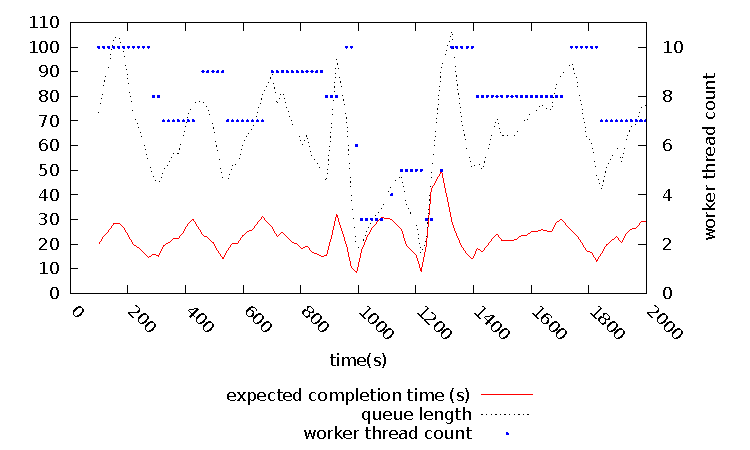
\includegraphics[width=0.5\textwidth]{../plot_data/plot1.pdf}
    \caption{Expected completion time, queue length and number of
    workers threads over time}
    \label{fig:exp1.1}
\end{figure}

Figure \ref{fig:exp1.3} shows the total expected sequential processing time (the
time required to empty the queue if there had only been one worker) and the
amount of worker threads. Both the amount of worker threads and the expected
sequential processing time follow the same pattern, showing how well the system
actually scales up and down.
\begin{figure}
    \centering  
    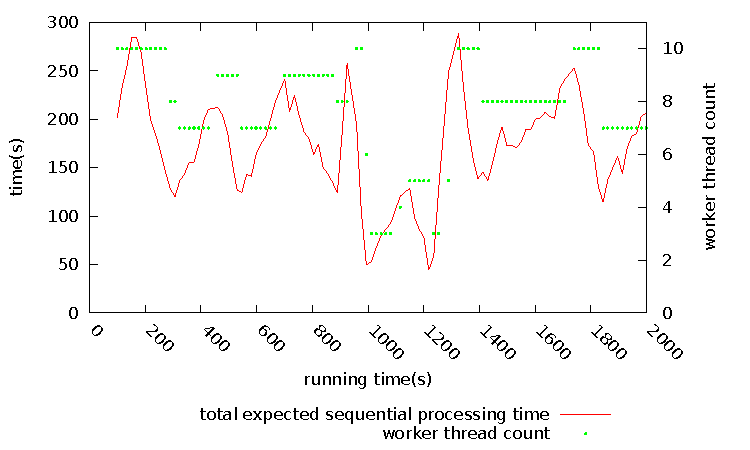
\includegraphics[width=0.5\textwidth]{../plot_data/plot3.pdf}
    \caption{Expected sequential processing time vs number of worker threads
    over time}
    \label{fig:exp1.3}
\end{figure}

The total sequential runtime of the experiment can be calculated by adding the
runtimes of all workers and the master node. This gives a total of 14000
seconds, thus 3.9 charged-time hours. At a total of 10 Euro-cents/ charged hour
the experiment cost a total of 39 cents. In this time about 4000 image tasks were
processed, giving us a total cost of 0.01 cents per image task.

% i. Charged-time = time that would have been charged using the
% Amazon EC2 timing approach (1-hour increments)
% ii. Charged-cost = cost that would have been charged using the
% Amazon EC2 charging approach, assuming 10 Euro-cents/charged hour
% iii. Service metrics of the experiment, such as runtime and response time of
% the service, etc.
% iv. (optional) Usage metrics of the experiment, such as per-VM and overall
% system usage and activity.


% \subsubsection{Experiment 2}
% \label{sssec:Experiment2}
% In this experiment the robustness of the system is tested. While the system is
% running the master VM's messaging queue and controller process are killed. This
% should cause the workers to send the \emph{AppState.ERROR} state to the head node (they
% lose their connection with the messaging queue and can't send acknowledgements).
% Also, it should cause the head node to delete the master and create a new
% master, as it doesn't receive \emph{Heartbeats} anymore.
% 
% Whether the scenario mentioned above conforms with the performance of the actual
% system can be tested by killing the message queue and the master runner tasks
% and by verifying that the head node responds correctly. The result of this
% experiment is shown below.
% 
% First, the system was brought to a stable state: all messages were consumed at the
% same rate at which they were processed. After this, the tasks on the master node
% were killed by connecting to the VM and killing the processes. The headnode no
% longer received a Heartbeat from the master, and all workers correctly reported
% they were in the ERROR state.
% 
% The head node responded by deleting the master VM, creating a new master VM and
% suspending all workers. The latter is done to reduce the cost - starting a new
% master can take a few minutes. As soon as the master node is in the
% \emph{AppState.READY} state the head node sends a \emph{AppCommand.INIT}
% command. The master node correctly replies with a \emph{AppState.RUNNING} state,
% causing the head node to resume all workers. After the workers verified they are
% running again they receive a new \emph{AppCommand.INIT} message containing the
% IP address of the new master node, allowing the workers to resume running.
% 
% This experiment took about 10 minutes using $4$ workers and $1$ master VM at a
% time. The total charged-time is one hour, which costs 10 Euro-cents.
% 
% \subsubsection{Experiment 3}
% \label{sssec:Experiment3}
% In this experiment another aspect of the robustness of the system is tested.
% Instead of killing both the master VM's messaging queue and its controller
% process only the messaging queue is killed.
% The main difference with \emph{Experiment 2} is that the workers should not send
% \emph{AppState.ERROR} messages to the head node - they can continue their work.
% Still, it should cause the head node to delete the master and create a new
% master, as it doesn't receive \emph{Heartbeats} anymore.
% 
% The experiment was started as described in section \emph{sssec:Experiment2}.
% After the master VM's controller was killed the workers indeed continue to send
% \emph{AppState.RUNNING} heartbeats to the head node. The head node no longer
% received a heartbeat from the master node, causing it to correctly delete the
% master VM, create a new master VM and suspend the workers.
% 
% The system performed exactly as required. It correctly identified that the
% master VM's controller crashed and deleted the VM. It suspended all workers and
% resumed them after the new master VM was running, and the controller
% initialized.
% 
% This experiment took about 10 minutes using $4$ workers and $1$ master VM at a
% time. The total charged-time is one hour, which costs 10 Euro-cents.

% describe the working environments (DAS, Amazon EC2, etc.), the general workload
% describe the experiments you have conducted to analyze each
% system feature, then analyze them; use one sub-section per experiment. For
% each experiment, describe the workload, present the operation of the system,
% and analyze the results. In the analysis, report:
% i. Charged-time = time that would have been charged using the
% Amazon EC2 timing approach (1-hour increments)
% ii. Charged-cost = cost that would have been charged using the
% Amazon EC2 charging approach, assuming 10 Euro-cents/charged hour
% iii. Service metrics of the experiment, such as runtime and response time of
% the service, etc.
% iv. (optional) Usage metrics of the experiment, such as per-VM and overall
% system usage and activity.

\section{Discussion}
\label{sec:Discussion}
Although NajNaf is relatively complex for an image resize
application because of the advanced requirements of the system, it proves to be
a viable alternative to the current system WantCloud BV is using. 

The experiments show that
NajNaf satisfies both (\namedref{nfr:elasticity}) and
(\namedref{nfr:response-time}). The cost of processing one image is relatively
low: section
\ref{sssec:experiment-result} shows the processing of a single image task (with a
processing time of three seconds) costs as little as 0.01 Euro-cents. Since the
system always needs exactly one active master node the cost of scaling a single
image becomes slightly less as the size of the queue increases: the overhead of
having the master node is spread out over more images. Thus when extrapolating
over the found results, 10.000 images can
be submitted for a total cost of 1 Euro, while the resizing of 10.000.000 images
costs less than a 1000 Euro.


Apart from the requirements that are shown to be met by the experiments, there
are several other features in the prototype that make the prototype meet all of its
requirements.

The head node keeps a log of all activities in the system. This log contains the
latest states of the applications, the average processing times of the workers,
the length of the messaging queue and many other statistics. The log itself is in
human-readable format, satisfying (\namedref{fr:monitoring}).

Whenever a worker node crashes the head node deletes the VM and creates a new
one. Since the worker only sends an acknowledgement after it has finished
processing the image task it is guaranteed that no image tasks are lost. This
satisfies both (\namedref{nfr:automation}) and (\namedref{nfr:reliability}).
Whenever the master node crashes a new master node is created, and all workers
are set to fetch image tasks from the new master. This also happens automatically,
again conforming with (\namedref{nfr:automation}).

Due to the slow-start algorithm workers only fetch image tasks when they are able
to actually process the image task. This conforms with
(\namedref{nfr:load-balancing}).

\section{Conclusion}
\label{sec:Conclusion}
In this paper the design of NajNaf was described - a system that tries to deal
with all the problems WantCloud BV's current system has. Experiments have been
conducted on a prototype of the system and together with sound reasoning we have shown that that the system
meets all the prototype requirements.

However, the prototype system does not contain all requirements, but provides a good base
for the production system. All production requirements can be achieved by
extending the prototype without exceptions. As a result we are convinced NajNaf
can play an important part in the future of WantCloud BV. We therefore recommend
WantCloud BV to choose for a cloud based solution, either off-the-shelf or
custom made.

\bibliographystyle{plain}
\bibliography{references}
\appendices
\section{Time sheet}
\label{sec:Time sheet}
    \begin{tabular}{|l|l|}
        \hline
        \textbf{Activity} & \textbf{Time Spent (hour)}\\
        \hline
        Thinking (design)& 30\\
        Developing &  90 \\
        Experimenting & 10 \\
        Analysis & 10 \\
        Writing(report) & 35 \\
        Wasted (setup etc.) & 30\\
        \hline
        \hline
        Total & 205\\
        \hline
    \end{tabular}\\

  The amount of time used for experimenting is fairly small compared to the
  other activities, this is mainly because the
  resource monitor was already in place and we only had to simulate workload for
  the system. Of the time spent on the experiments about 70\% of the time was
  used for debugging and the remaining time was used to build a workload
  simulator and actually run the experiments.


\end{document}


